\xiti
\begin{xiaotis}

\xiaoti{画出下列几何体的视图(可以省略某些视图)。}

\begin{figure}[htbp]
    \centering
    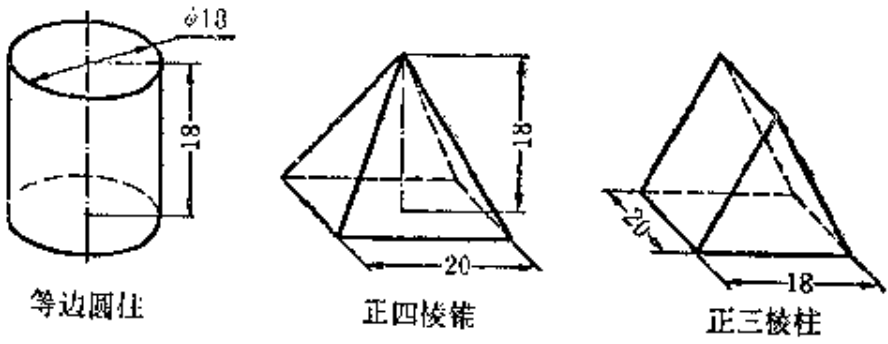
\includegraphics[width=11cm]{../pic/czjh2-ch8-xiti30-01-1.png}
    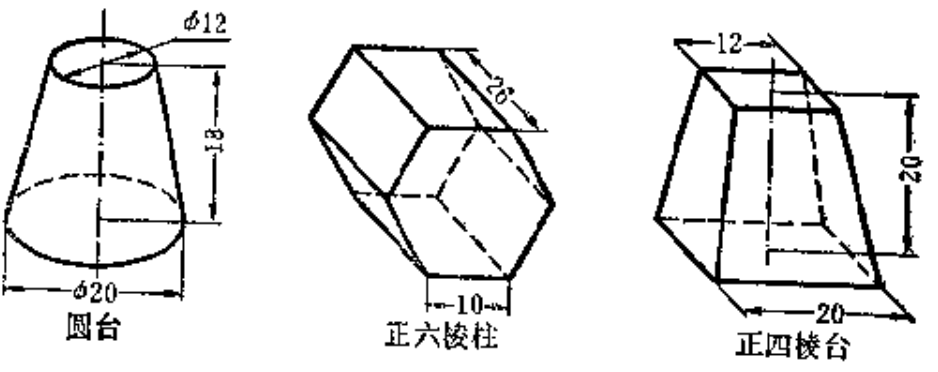
\includegraphics[width=11cm]{../pic/czjh2-ch8-xiti30-01-2.png}
    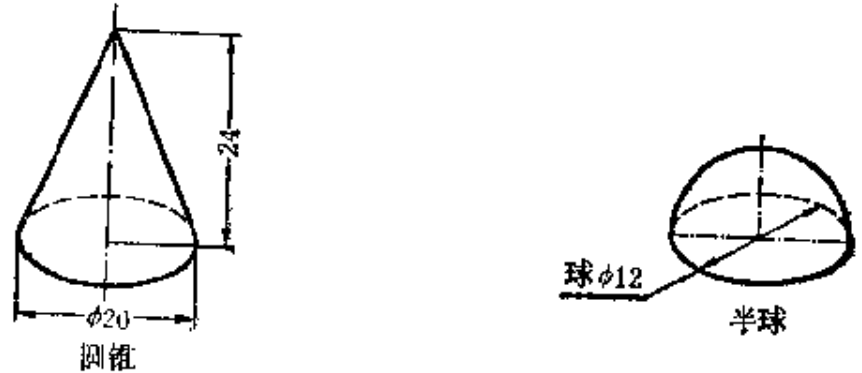
\includegraphics[width=11cm]{../pic/czjh2-ch8-xiti30-01-3.png}
    \caption*{(第 1 题)}
\end{figure}


\xiaoti{以比例尺 $1.5:1$ 画出下列零件的三视图(提示:比例尺 $1.5:1$ 就是放大成原来的 1.5 倍)。}

\begin{figure}[H]%[htbp]
    \centering
    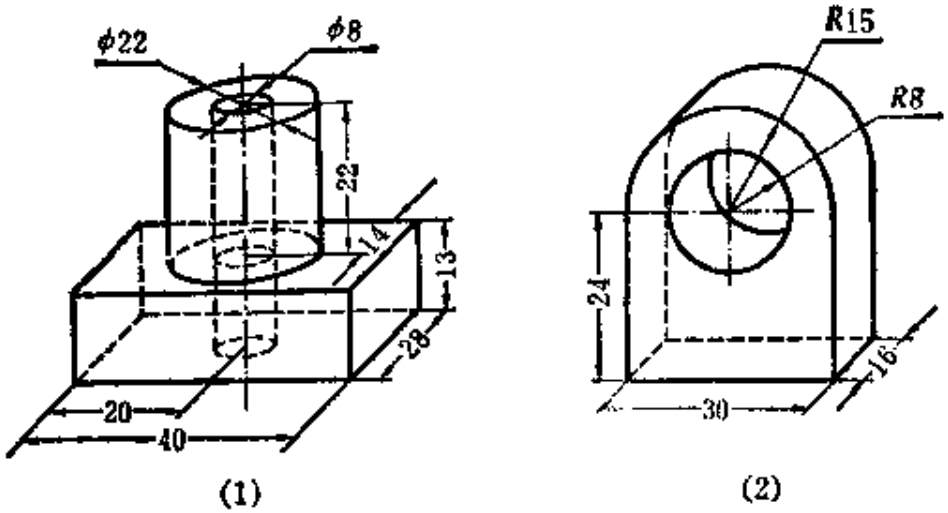
\includegraphics[width=11cm]{../pic/czjh2-ch8-xiti30-02.png}
    \caption*{(第 2 题)}
\end{figure}

\xiaoti{下列视图有没有错误?为什么?错的如何改正?}

\begin{figure}[htbp]
    \centering
    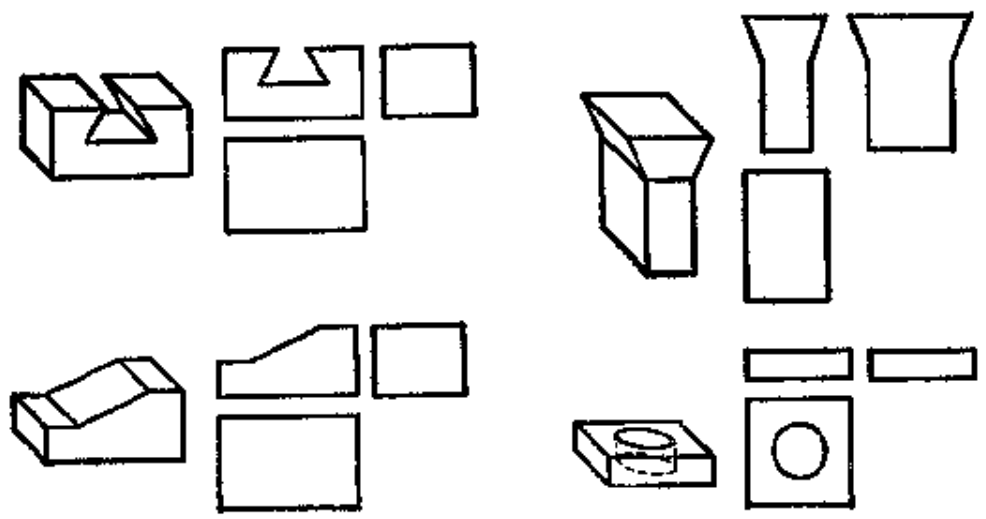
\includegraphics[width=11cm]{../pic/czjh2-ch8-xiti30-03.png}
    \caption*{(第 3 题)}
\end{figure}

\end{xiaotis}

